% !Mode:: "TeX:UTF-8"
% !TEX program  = xelatex
\documentclass[a4paper]{article}
\usepackage{amsmath}
\usepackage{amssymb}
\usepackage{ctex}
\usepackage{graphicx}
%\usepackage{braket}
\usepackage[european]{circuitikz}
\usepackage{multirow}
\usepackage{geometry}
\usepackage{float}
\geometry{left=2.5cm,right=2.5cm,bottom=2.5cm,top=2.5cm}
\title{物理化学拓展实验: 电导率测定氯化银解离平衡反应热力学常数}
\author{薛明怡\quad 151250177\quad 化学化工学院}
\date{\today}
\begin{document}
\maketitle
%%\tableofcontents
%%\bibliographystyle{unsrt}
\section{实验目的}
\begin{enumerate}
	\item 掌握电导法测定电解质溶液的摩尔电导.
	\item 了解电导率的应用.
\end{enumerate}
\section{实验原理}
\subsection{电导率}
电导率是电阻率($\rho$)的倒数, 是衡量物质导电能力的基本性质, 通常用希腊字母$\sigma$表示.
\begin{equation}
	\centering
	\begin{aligned}
		\rho &= R\frac{A}{l}\\
		\kappa &= \frac{1}{\rho}= G\frac{l}{A}\\
	\end{aligned}
\end{equation}
\begin{figure}[H]
	\centering
	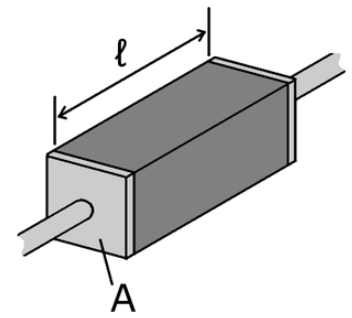
\includegraphics[width=0.2\paperwidth]{fig/resistivity_conductivity_definition.PNG}
	\caption{电阻率和电导率的定义}
\end{figure}
其中, $R$是均匀样品的电阻, $l$是样品的长度, $A$是样品截面面积.
电阻率的单位是$\Omega\cdot m$, 电导率的单位是$S/m$.
\par
更一般的标量定义方式是,
\begin{equation}
	\centering
	\begin{aligned}
		\rho &= \frac{E}{J}\\
		\kappa &= \frac{1}{\rho} = \frac{J}{E}\\
	\end{aligned}
\end{equation}
其中, $E$是电场强度, $J$是电流密度. 例如, 
橡胶是一种具有高电阻率低电导率的材料, 因为将橡胶放置
在强电场中几乎不产生电流. 相反, 铜是一种具有低电阻率高电导率
的材料, 因为即使一个小的电场也能产生大的电流通过.
\par
上述定义很自然的可以导出电阻率和电导率的张量定义, 
张量定义是一种完全广义的定义方式, 但由于定义最为复杂因此只在各向异性
情景中被使用. 如果材料不是各向异性的, 用上述两种简单的表达式即可. 
如石墨在微观上由一层层的石墨烯构成, 电流可以轻易的在每一层上通过, 
但是无法轻易的从一层流到与它相邻的另一层. 在后面的情景下, 
电流的流向不完全与电场方向一致, 从而需要使用电导率的张量定义.
\begin{equation}
	\centering
	\begin{aligned}
		\mathbf{J} &= \mathbf{\kappa} \mathbf{E}\\
		\left[\begin{matrix}
			J_{x}\\
			J_{y}\\
			J_{z}\\ 
	  \end{matrix}\right]
	  &=
		\left[\begin{matrix}
			\kappa_{xx} & \kappa_{xy} & \kappa_{xz} \\
			\kappa_{yx} & \kappa_{yy} & \kappa_{yz} \\
			\kappa_{zx} & \kappa_{zy} & \kappa_{zz} 
		\end{matrix}\right] 
		\left[\begin{matrix}
			  E_{x}\\
			  E_{y}\\
			  E_{z}\\ 
		\end{matrix}\right]
	\end{aligned}
\end{equation}
\subsection{摩尔电导率}
摩尔电导率$\Lambda_{m}$是指把含有$1mol$电解质的溶液置于相距为单位距离
的电导池的两个平行电极之间, 这时所具有的电导. 由于对不同的电解质均取$1mol$
但所取溶液的体积$V_{m}$将随浓度而改变. 设$c$是电解质溶液的浓度(单位为$mol\cdot m^{-3}$), 
则含$1mol$电解质的溶液的体积$V_{m}$应等于$\frac{1}{c}$, 根据电导率$\kappa$的定义, 
摩尔电导率$\Lambda_{m}$,
\begin{equation}
	\Lambda_{m} = \kappa V_{m} = \frac{\kappa}{c}\\
\end{equation}
% \subsection{电导池常数}
% 电导池中两极之间的距离$l$和涂有波黑的电极面积$A$是很难测量的, 通常是把已知电阻率的溶液
% (通常是一定浓度的$KCl$溶液)注入电导池, 就可确定$\frac{l}{A}$值, 这个值被称为电导池常数
% $K_{cell}$,
% \begin{equation}
% 	K_{cell} = \frac{1}{\rho}R = \kappa R\\
% \end{equation}
\subsection{氯化银的溶解平衡与溶度积}
$AgCl$为难溶盐, 在水中溶解度小导致浓度无法用普通的滴定法测定, 但可以用电导法求得. 
首先先制备饱和$AgCl$溶液, 测量溶液的电导率$\kappa(solution)$,
\begin{equation}
	\kappa(AgCl) = \kappa(solution) - \kappa(H_{2}O)\\
\end{equation}
摩尔电导率的计算公式为,
\begin{equation}
	\Lambda_{m}(AgCl) = \frac{\kappa(AgCl)}{c(AgCl)}\\
\end{equation}
由于难溶盐的溶解度很小, 溶液极稀, 所以可以认为$\Lambda_{m} \approx \Lambda_{m}^{\infty}$, 
而$\Lambda_{m}^{\infty}$的值可以由离子无限稀释摩尔电导率相加而得, 
\begin{equation}
	\Lambda_{m}^{\infty}(AgCl) = 	\Lambda_{m}^{\infty}(Ag^{+}) +	\Lambda_{m}^{\infty}(Cl^{-})\\
\end{equation}
由式(6)可以求得饱和$AgCl$溶液的浓度, 
\begin{equation}
	\centering
	\begin{aligned}
		c(AgCl) &= \frac{\kappa(AgCl)}{\Lambda_{m}(AgCl)}\\
				&=\frac{\kappa(AgCl)}{\Lambda_{m}^{\infty}(AgCl)}\\
				&=\frac{\kappa(AgCl)}{\Lambda_{m}^{\infty}(Ag^{+}) +	\Lambda_{m}^{\infty}(Cl^{-})}\\
	\end{aligned}
\end{equation}
最后根据下式可以得到$AgCl$的溶度积.
\begin{equation}
	\centering
	\begin{aligned}
		K_{sp} &= a_{Ag^{+}} \cdot a_{Cl^{-}}\\
		&= \gamma_{\pm}^{2} \cdot 
		\frac{c_{Ag^{+}} c_{Cl^{-}}}{C^{\theta 2}} \\
		&\approx \frac{c_{Ag^{+}} c_{Cl^{-}}}{c_{\theta}^{2}} \\
		&=(\frac{c_{AgCl}}{c_{\theta}})^{2}\\
	\end{aligned}
\end{equation}
\subsection{解离平衡热力学常数}
氯化银解离平衡反应如下, 
\begin{equation}
	AgCl \to Ag^{+} + Cl^{-}
\end{equation}
假定在温度变化范围不大的情况下, 标准摩尔解离焓和标准摩尔解离熵可以视为常数, 
因此$lnK_{sp}$与$\frac{1}{T}$成一次函数关系, 并可求得在$298.15K$时
解离平衡的标准摩尔吉布斯自由能.
\begin{equation}
	\centering
	\begin{aligned}
		\Delta_{r}G_{m}^{\theta} &= -RTlnK_{sp}\\
		&=\Delta_{r}H_{m}^{\theta} - T\Delta_{r}S_{m}^{\theta}\\
		lnK_{sp} &= -\frac{\Delta_{r}H_{m}^{\theta}}{RT} + \frac{\Delta_{r}S_{m}^{\theta}}{R}\\
	\end{aligned}
\end{equation}
\section{仪器与药品}
\begin{enumerate}
    \item \textbf{仪器:} 电导率仪, 恒温槽, 吸滤瓶, $50mL$烧杯
    \item \textbf{药品:} $0.1mol/L~AgNO_{3}$溶液, $0.1mol/L~KCl$溶液, 电导水
\end{enumerate}
\section{实验步骤}
\subsection{$AgCl$的制备}
\begin{itemize}
	\item 称取$0.075g$左右KCl固体溶解在$20mL$蒸馏水中, 配制成约$0.1mol/L$的KCl溶液;
	向上述溶液中加入$10mL$ $0.1mol/L~AgNO_{3}$溶液于烧杯中.
	\item 用吸滤瓶过滤溶液, 滴加电导水抽滤3次. 
	% \item 称量制得的白色固体, 并将其保存在棕色试剂瓶中或立即使用.
\end{itemize}
\subsection{测定饱和$AgCl$溶液电导率}
\begin{itemize}
	\item 校正电导率仪.
	\item 取少量新制的$AgCl$固体溶解在试管中, 加入$20mL$电导水, 
	搅拌, 在$25^\circ$C恒温槽中静置约$15min$, 达到溶解平衡.
	\item 测定该温度下饱和$AgCl$溶液和电导水的电导率. 
	\item 重复上述步骤, 继续测定$30^\circ$C, $35^\circ$C, $40^\circ$C
	下饱和$AgCl$溶液和电导水的电导率, 获得升温曲线.
	\item 测定$40^\circ$C, $35^\circ$C, $30^\circ$C, $25^\circ$C
	下饱和$AgCl$溶液和电导水的电导率, 获得降温曲线; 
	降温实验中可以将静置时间设置为$10$min.
	\item 对比上述曲线的
	\item 用电导法测量的$AgCl$溶度积可与电动势测定实验中的值进行对比.
\end{itemize}
\newpage
\section{数据处理}
\subsection{电导水电导率的温度曲线}
表3直线拟合结果如下,
\begin{figure}[H]
	\centering
	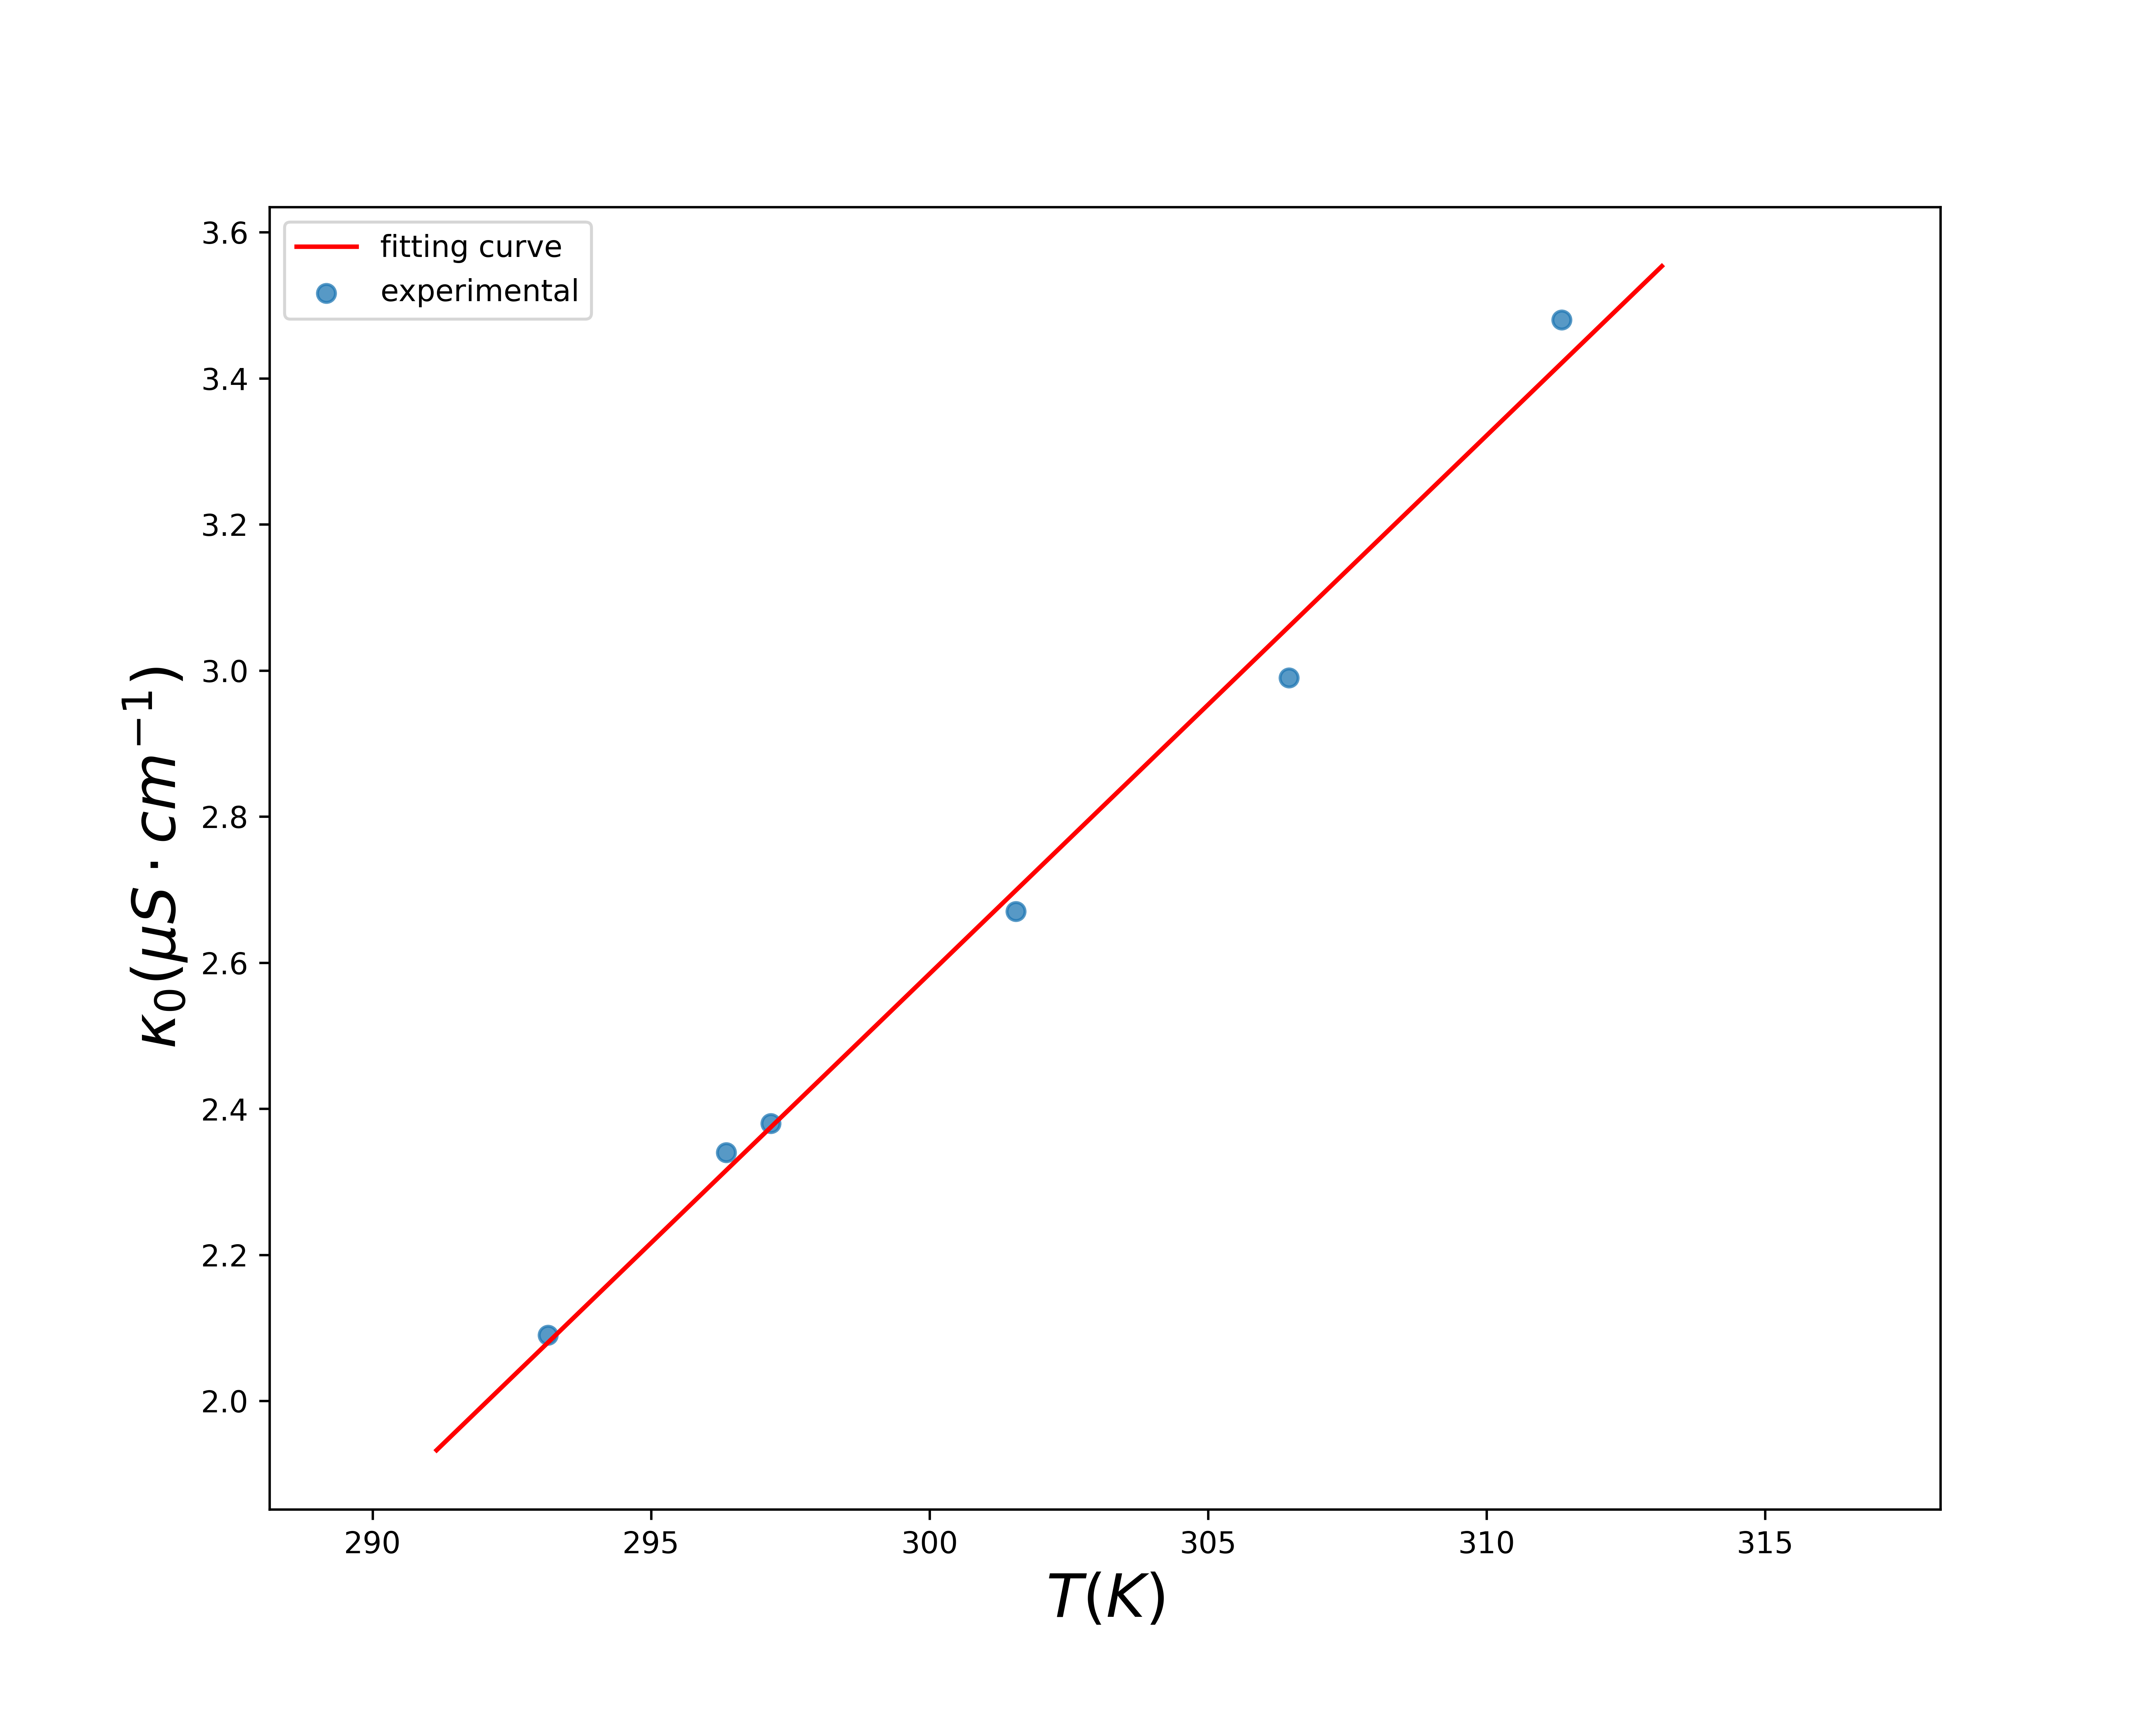
\includegraphics[width = 0.5\linewidth]{fig/H2O.png}
	\caption{电导水电导率-温度曲线}
	\label{}
\end{figure}
\begin{equation}
	\centering
	\begin{aligned}
		\kappa_{0} &= 7.3690\times 10^{-2} T - 19.5223\\
		R^{2} &= 0.9923\\
	\end{aligned}
\end{equation}
\subsection{饱和AgCl溶液电导率的温度曲线}
\begin{table}[H]
	\caption{实验数据处理表}
	\begin{center}
		\begin{tabular}{lllll}
			\hline
			温度/K 	&$\kappa_{sol, AgCl}$/$\mu S\cdot cm^{-1}$ 
			& $\kappa_{0}$计算值/$\mu S\cdot cm^{-1}$& $\kappa_{AgCl}$/$\mu S\cdot cm^{-1}$
			&$K_{sp}$计算值\\
			\hline
			309.95&4.29&3.32&0.97&$4.94\times 10^{-7}$ \\
			308.15&4.22&3.18&1.03&$5.60\times 10^{-7}$ \\
			308.05&4.25&3.18&1.07&$6.01\times 10^{-7}$ \\
			306.35&4.15&3.05&1.10&$6.30\times 10^{-7}$ \\
			306.25&4.12&3.04&1.07&$6.04\times 10^{-7}$ \\
			304.65&4.03&2.93&1.10&$6.36\times 10^{-7}$ \\
			302.65&3.90&2.78&1.12&$6.56\times 10^{-7}$ \\
			300.95&3.75&2.65&1.10&$6.28\times 10^{-7}$ \\
			299.05&3.61&2.51&1.10&$6.28\times 10^{-7}$  \\
			298.55&3.59&2.48&1.11&$6.47\times 10^{-7}$  \\
			296.65&3.45&2.34&1.11&$6.47\times 10^{-7}$  \\
			295.15&3.32&2.23&1.09&$6.25\times 10^{-7}$ \\
			294.95&3.30&2.21&1.09&$6.19\times 10^{-7}$ \\
			294.05&3.23&2.15&1.08&$6.14\times 10^{-7}$ \\
			293.05&3.17&2.07&1.10&$6.30\times 10^{-7}$  \\
			\hline
		 \end{tabular}
	\end{center}
\end{table}
\begin{equation}
	\centering
	\begin{aligned}
		\ln K_{sp} &= \ln  (\frac{c_{AgCl}}{c^{\theta}})^{2}\\
		&=2\ln(\frac{\kappa_{AgCl}}{\Lambda^{\infty}_{m}(Ag^{+})+\Lambda^{\infty}_{m}(Cl^{-})} / c^{\theta})\\
		&=-\frac{\Delta_{r}H^{\theta}_{m}}{RT} + \frac{\Delta_{r}S^{\theta}_{m}}{R}\\
		\ln  (\frac{c_{AgCl}}{c^{\theta}}) &= -\frac{\Delta_{r}H^{\theta}_{m}}{2RT} + \frac{\Delta_{r}S^{\theta}_{m}}{2R}\\
		&= \frac{k}{T} + b\\
		\Delta_{r}H^{\theta}_{m} &= -2kR\\
		\Delta_{r}S^{\theta}_{m} &= 2bR\\
		\Lambda^{\infty}_{m}(Ag^{+}) &= 61.92 \times 10^{-4} S\cdot m^{2} \cdot mol^{-1}\\
		\Lambda^{\infty}_{m}(Cl^{-}) &= 76.34 \times 10^{-4} S\cdot m^{2} \cdot mol^{-1}\\
	\end{aligned}
\end{equation}

\begin{figure}[H]
	\centering
	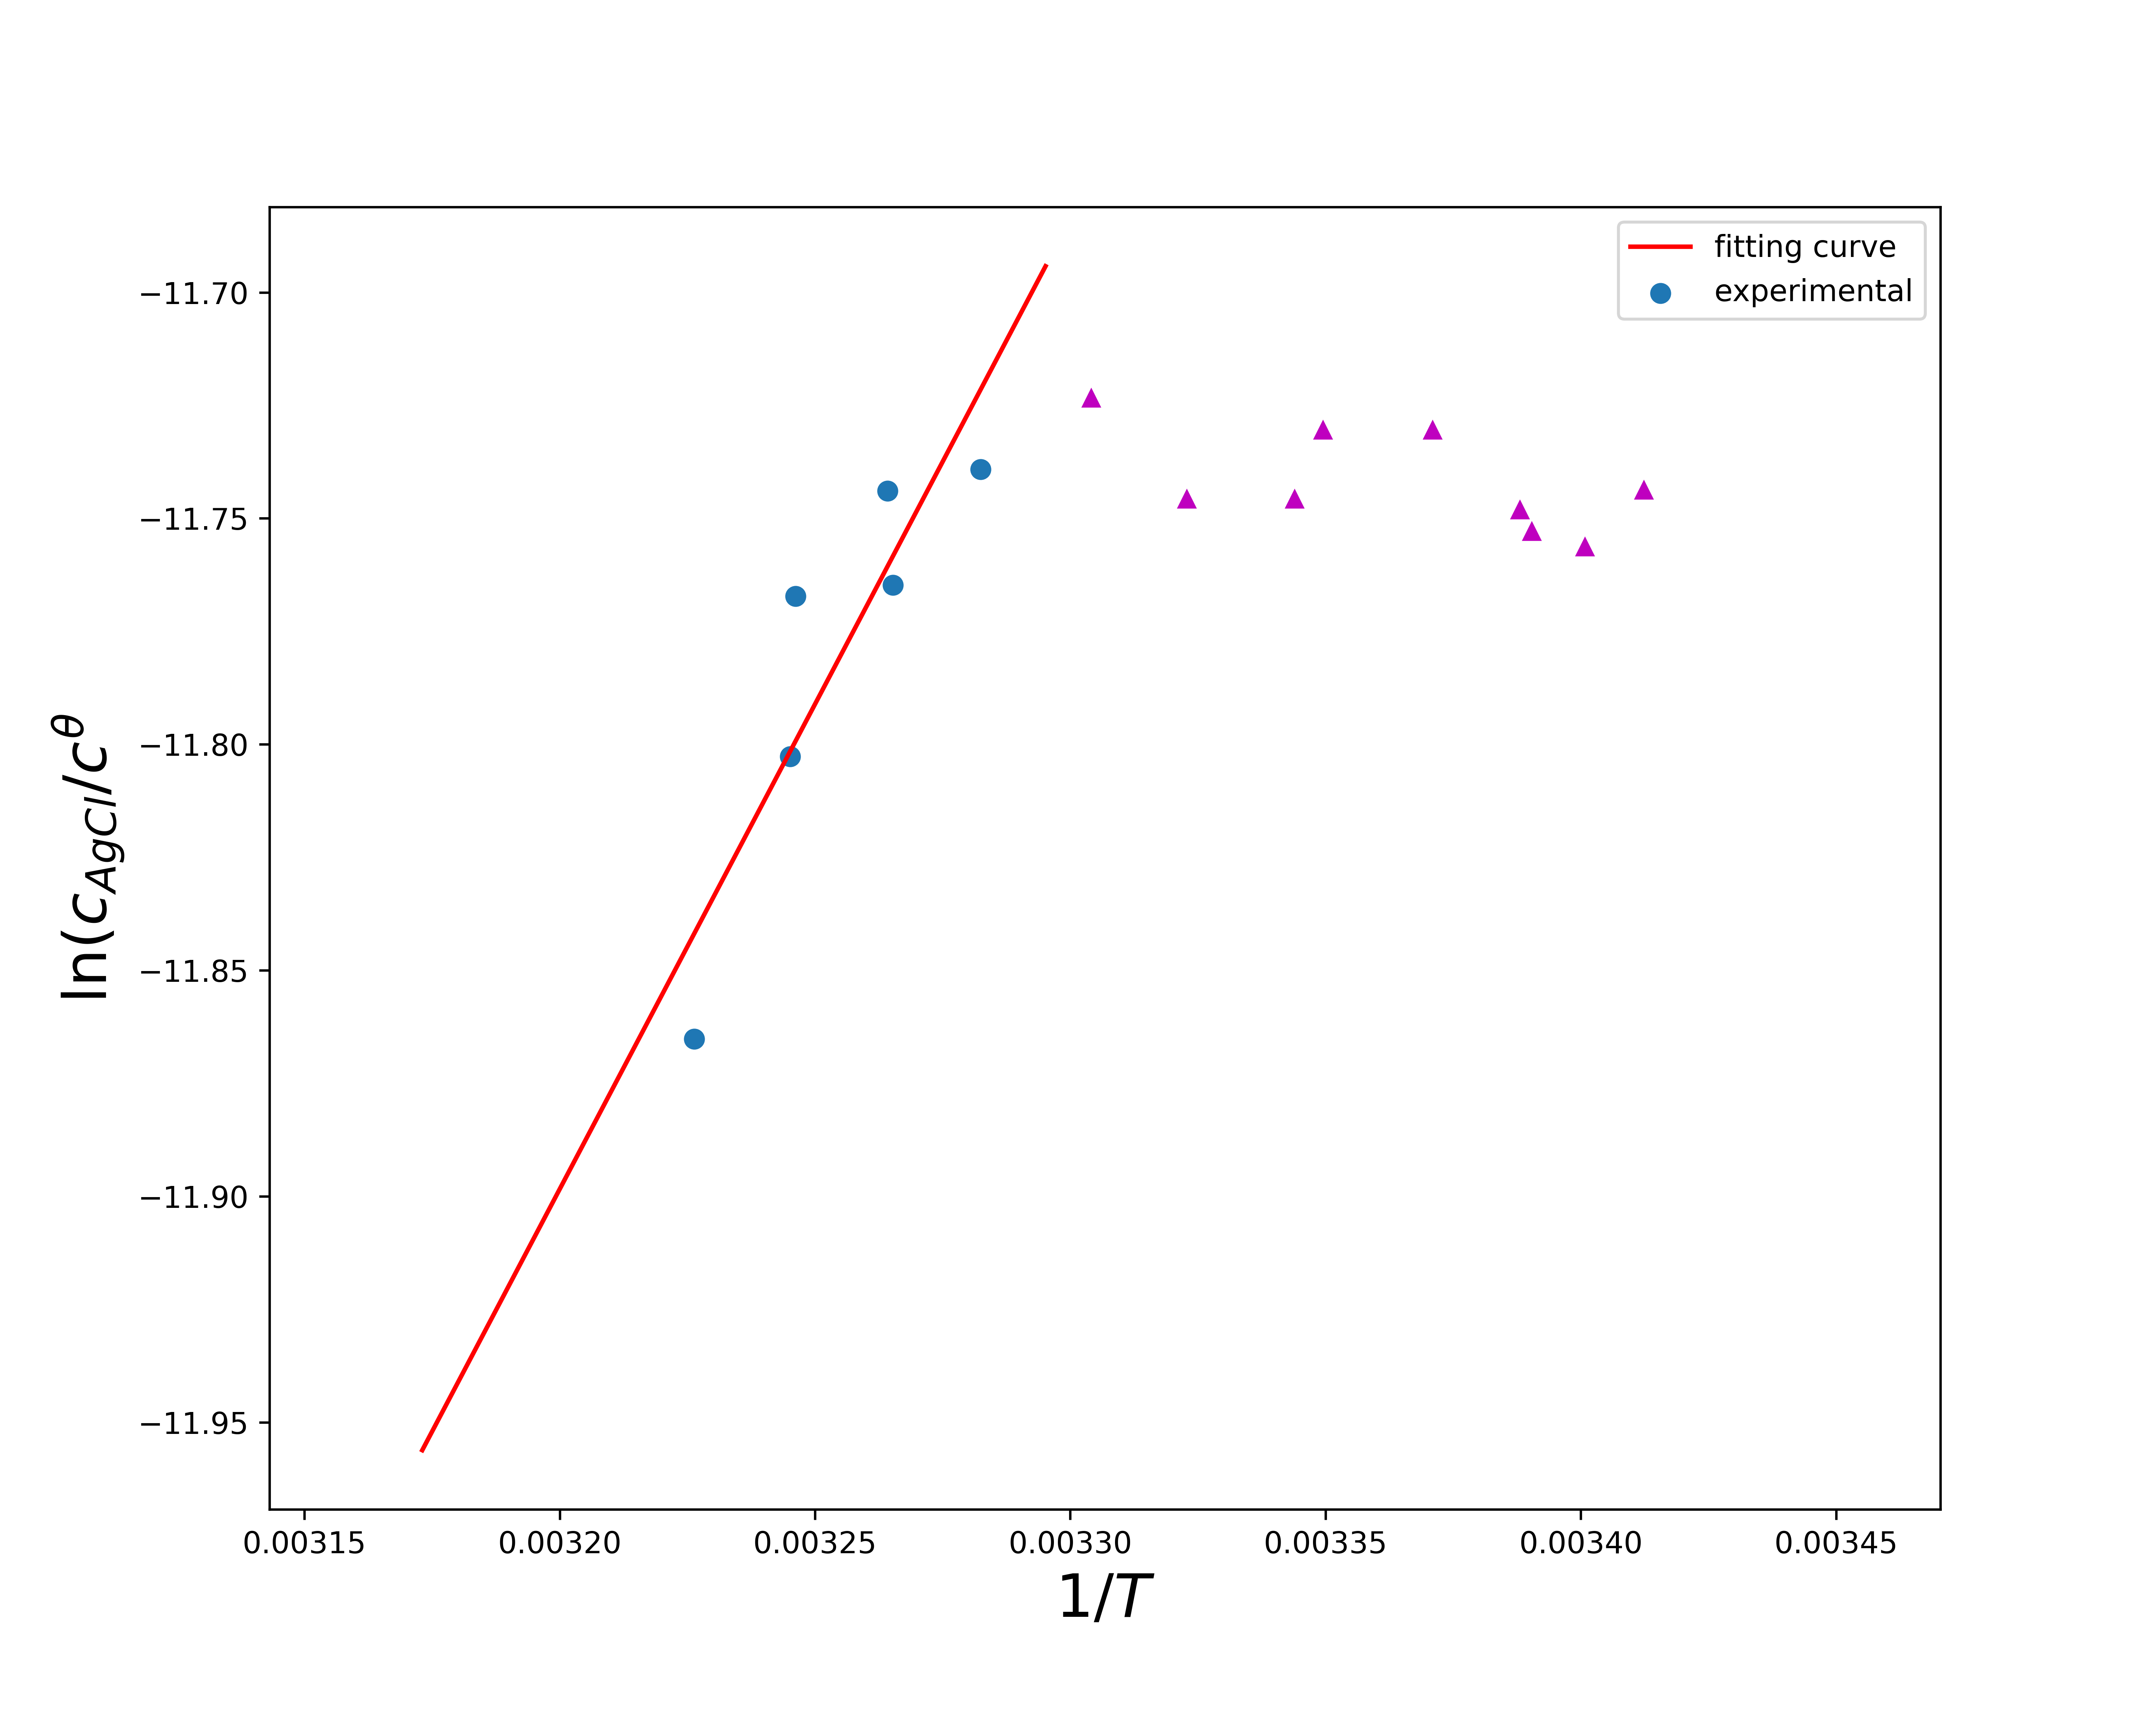
\includegraphics[width = 0.5\linewidth]{fig/high.png}
	\caption{$\ln(c_{AgCl}/c^{\theta})$-$\frac{1}{T}$高温区(32-40$^\circ$C)曲线}
	\label{}
\end{figure}
\begin{equation}
	\centering
	\begin{aligned}
		\ln(c_{AgCl}/c^{\theta}) &= 2.1455\times 10^{3} \times \frac{1}{T} - 18.7641\\
		R^{2} &= 0.8028 \\
		\Delta_{r}H^{\theta}_{m} &= -2kR \\
		&= -2\times 2.1455\times 10^{3} \times 8.314\\
		&= -35.68 kJ\cdot mol^{-1}\\
		\Delta_{r}S^{\theta}_{m} &= 2bR\\
		&=2\times (-18.7641) \times 8.314\\
		&= -312.0 J\cdot mol^{-1}
	\end{aligned}
\end{equation}
\par
数据分析见第6部分.
\begin{figure}[H]
	\centering
	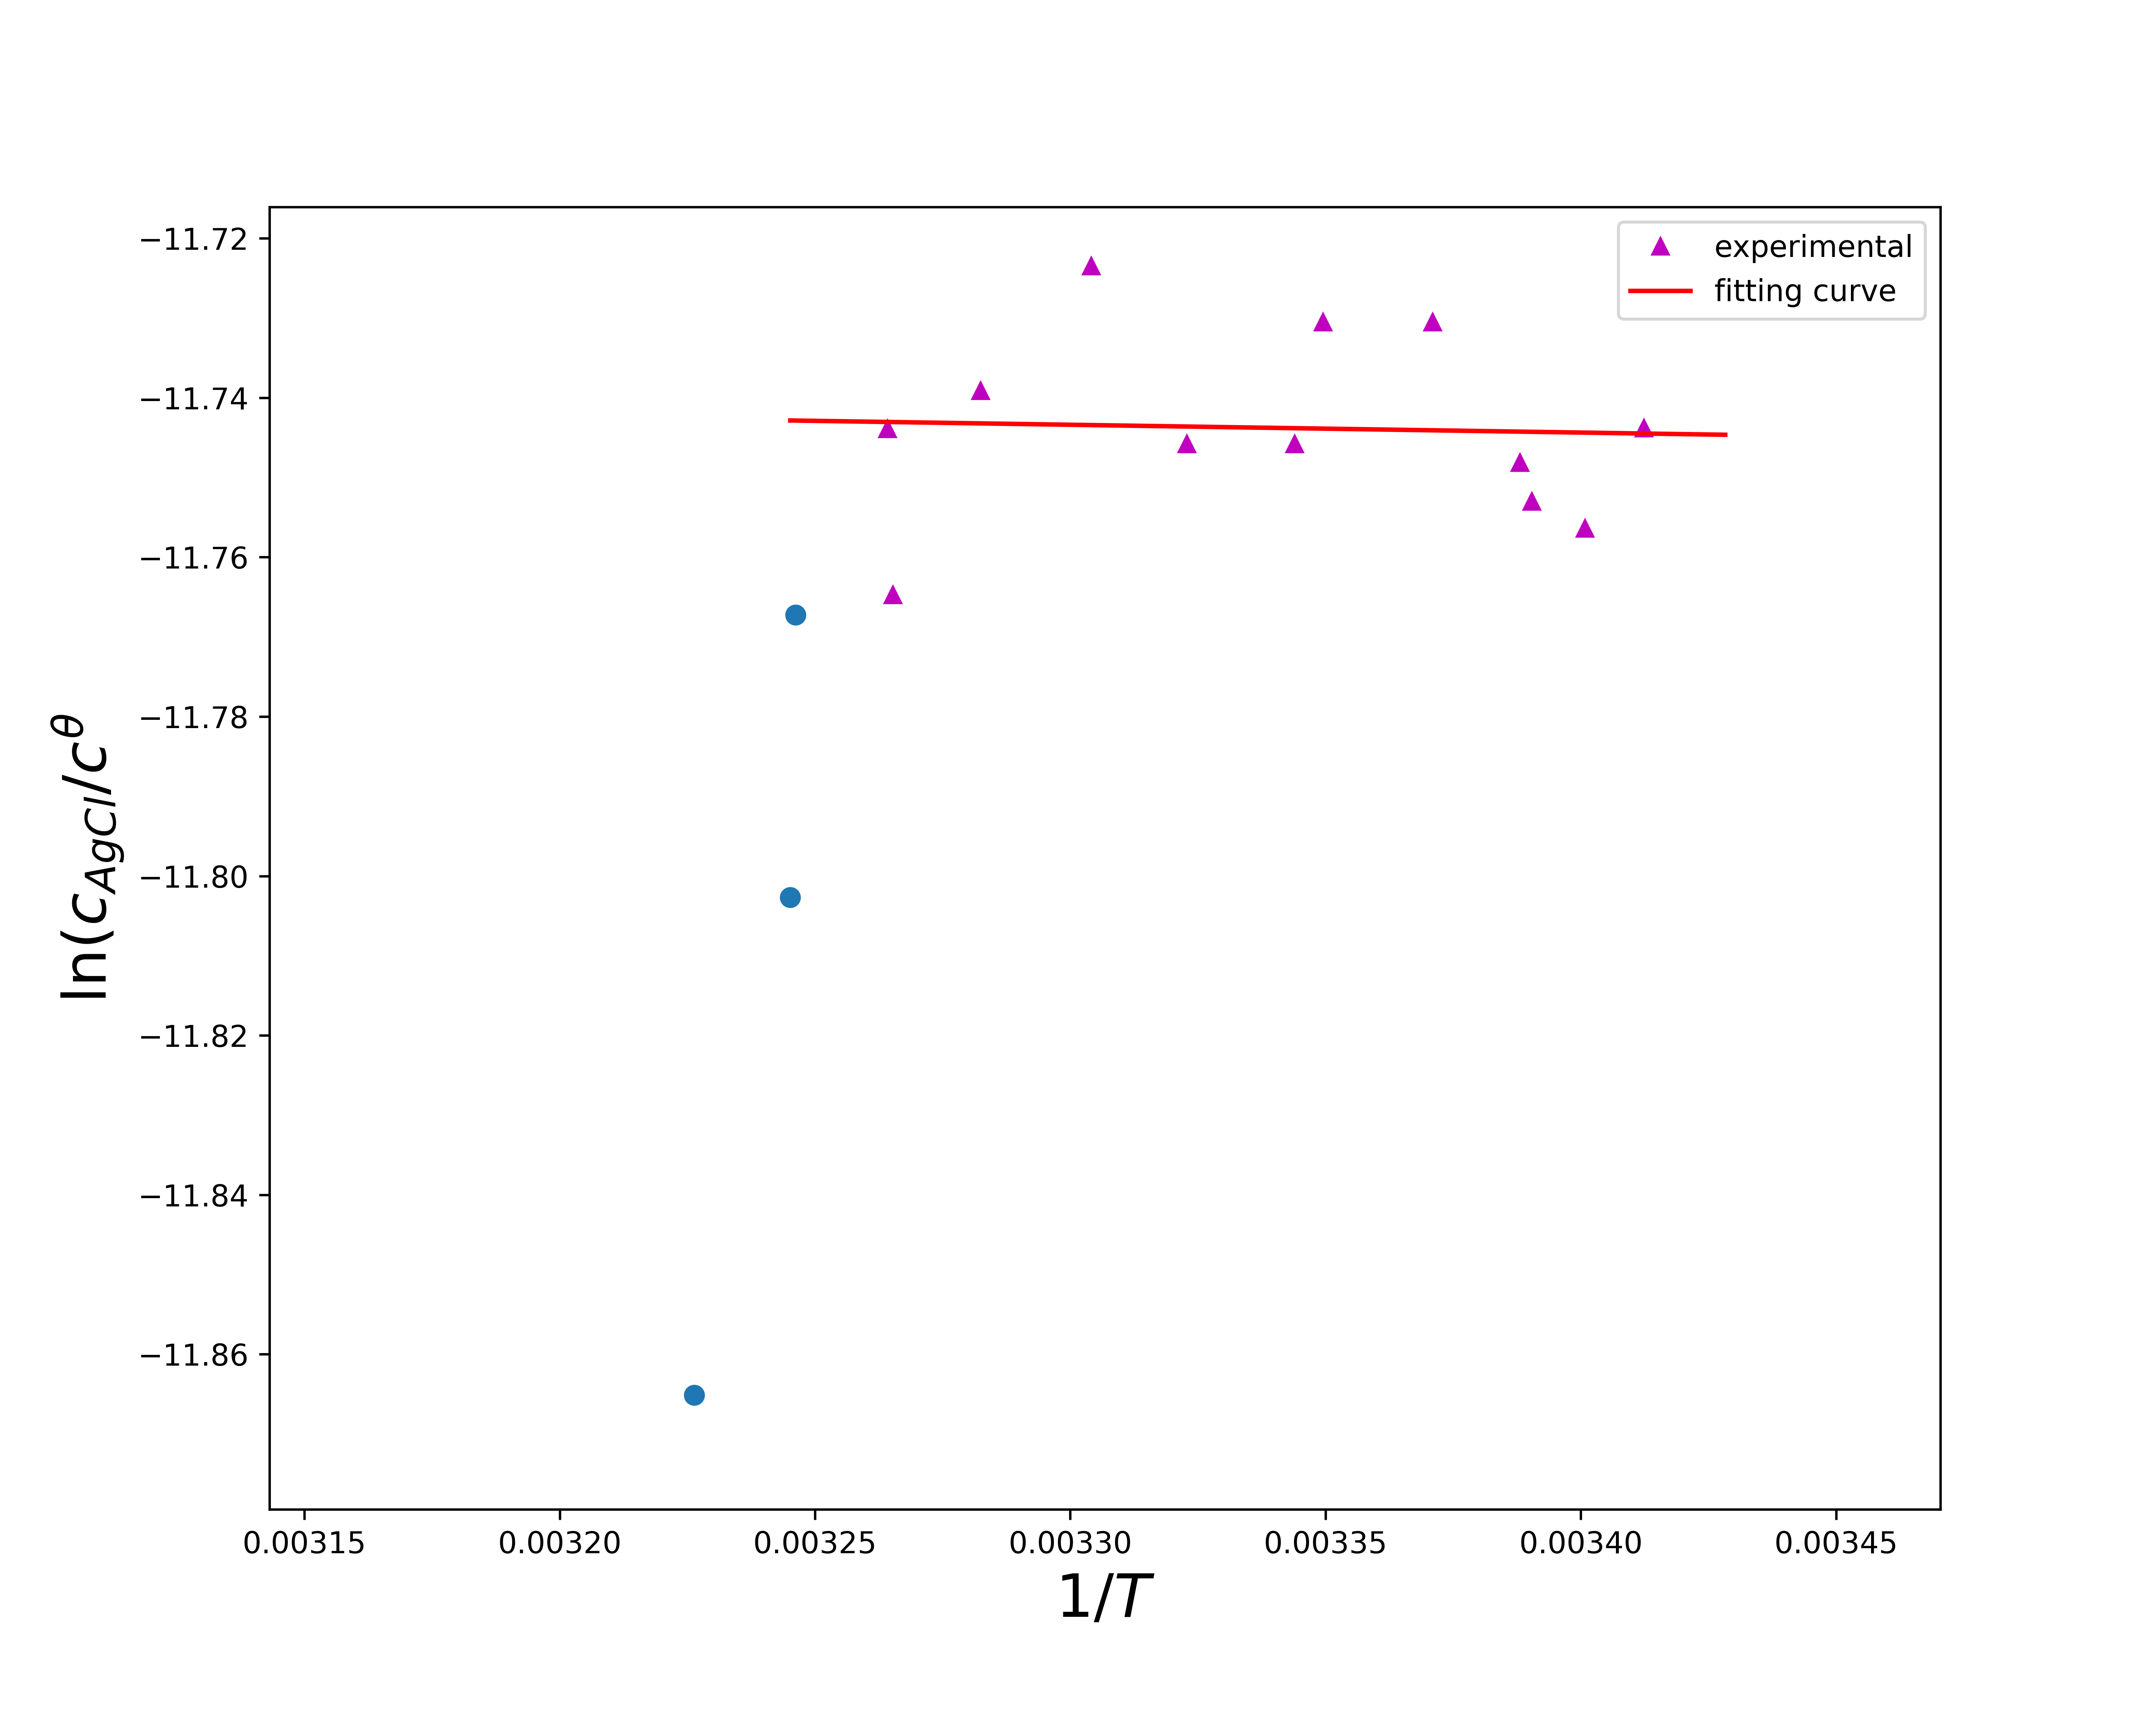
\includegraphics[width = 0.5\linewidth]{fig/low.png}
	\caption{$\ln(c_{AgCl}/c^{\theta})$-$\frac{1}{T}$低温区(20-30$^\circ$C)曲线}
	\label{}
\end{figure}
\begin{equation}
	\centering
	\begin{aligned}
		\ln(c_{AgCl}/c^{\theta}) &= -9.7942\times \frac{1}{T} - 11.7111\\
		R^{2} &= 0.0020
	\end{aligned}
\end{equation}
\par
低温区实验数据线性较差, 因此不使用低温区数据进行沉淀解离平衡热力学常数的计算. 
线性差的原因见第6部分.

\section{讨论与分析}
\begin{enumerate}
	\item 在制备AgCl的过程中, 新制的氯化银是白色的, 
	抽滤润洗多次后氯化银表面发灰, 表层的银离子很有可能已经被氧化.
	\item 电导水电导率与溶液温度的关系线性较好, $R^{2} = 0.9923$, 因此在$20^\circ$C - $40^\circ$C温度范围内, 
	电导水的电导率用$\kappa_{0} = 7.3690\times 10^{-2}T - 19.5223$计算得到.
	\item 根据$\kappa_{AgCl}$可以求出各温度下AgCl的溶度积$K_{sp}$, 
	本实验计算得到的溶度积在$10^{-7}$数量级, 而查表得到的298K时AgCl的溶度积为$1.56\times 10^{-10}$, 
	相差3个数量级. 由于电导率仪的示数为$0.01 \mu S\cdot cm^{-1}$, 
	因此精度为$0.1 \mu S\cdot cm^{-1} = 10^{-5} S\cdot m^{-1}$, 
	$K_{sp} = (c_{AgCl}/C^{\theta})^{2} = (10^{-5} / 10^{-4} / 10^{3})^{2} = 10^{-8}$, 
	因此理论上用FE30电导率仪只能测量溶度积大于$10^{-8}$数量级的难溶物, 
	为了测量$AgCl$的溶度积需要用精度更高的电导率仪. 
	\item 在高温区($32^\circ$C - $40^\circ$C)测得氯化银沉淀溶解
	平衡的标准摩尔焓变为$\Delta_{r}H^{\theta}_{m} = -35.68 kJ\cdot mol^{-1}$, 
	标准摩尔熵变为$\Delta_{r}S^{\theta}_{m} = -312.0 J\cdot mol^{-1}$; 
	表观表现为随着温度的升高AgCl的溶解度变小, 沉淀解离平衡是熵减反应, 与直觉不符.\\
	考虑到离子水解, 我们需要进一步测定$Ag^{+}$水解度与温度的关系曲线, 
	如果随着温度的升高银离子水解程度增大, 则可能解释本实验中高温区的数据,
	否则说明离子浓度小于仪器精度造成了系统误差.
	\item 在低温区($20^\circ$C - $30^\circ$C)溶解度几乎不随温度发生变化, 
	我认为很有可能是由于温度低平衡时间短, 氯化银溶解后来不及扩散到整个体系中形成均匀溶液造成的; 
	可以将体系中加入机械搅加快离子扩散平衡.
	\item 总体而言, 使用精度更高的电导率仪, 电导法能够定性的给出单一温度点AgCl的溶度积; 
	但由于Ag是高周期元素, $Ag^{+}$存在氧化/水解等耦合反应, 因此AgCl的溶解平衡反应十分复杂; 
	此外实验过程中发现电导水在开放的体系中很容易溶解
	空气中的二氧化碳等杂质, 造成电导率的变化, 不太适合用于需要变温和长时间测量的实验; 
	实验原理中对``沉淀溶解平衡标准摩尔焓变在一定温度范围内是常数''和
	``离子的无限摩尔电导率在一定温度范围内变化不大''的假设也比较粗糙.
	\item 本次实验从最终结果上看不是很成功, 
	最大的意义在于探索了电导法测定难溶物溶解度的适用范围:
	\begin{itemize}
		\item 避免离子氧化和水解带来的误差, 最好选用氧化能力较弱的一价阳离子的难溶盐;
		\item 考虑到FE30电导率仪的精度, 最好选用溶度积大于$10^{-8}$的难溶盐;
		\item 在体系中引入机械搅拌加快离子扩散过程;
		\item 可以使用离心机分离沉淀, 避免对溶液电导产生影响;
		\item 由于电导水在敞开体系中电导率变化很大, 因此本次实验如需长时间测定需要引入氮氛.
	\end{itemize}
\end{enumerate}
\newpage
\section*{原始数据记录}
\begin{table}[H]
	\caption{电导率测定实验数据--升温}
	\begin{center}
		\begin{tabular}{llll}
			\hline
			恒温槽温度/$^\circ$C	&电导率仪测量温度/$^\circ$C 	&饱和$AgCl$溶液电导率$\kappa$/$\mu S\cdot cm^{-1}$& 电导水电导率$\kappa_{0}$/$\mu S\cdot cm^{-1}$\\
			\hline
			25&23.9&2.22&1.59\\

			30&28.8&2.05&1.87\\

			35&33.5&2.44&2.17\\

			38&36.5&3.33&2.78\\

			40&38.7&3.66&3.27\\
			\hline
		 \end{tabular}
	\end{center}
\end{table}
\begin{table}[H]
	\caption{电导率测定实验数据--降温}
	\begin{center}
		\begin{tabular}{lll}
			\hline
			恒温槽温度/$^\circ$C	&电导率仪测量温度/$^\circ$C 	&饱和$AgCl$溶液电导率$\kappa$/$\mu S\cdot cm^{-1}$\\
			\hline
			38&36.8&4.29\\
			36&35.0&4.22\\
			36&34.9&4.25\\
			34&33.2&4.15\\
			34&33.1&4.12\\
			32&31.5&4.03\\
			30&29.5&3.90\\
			28&27.8&3.75\\
			26&25.9&3.61\\
			26&25.4&3.59\\
			24&23.5&3.45\\
			22&22.0&3.32\\
			22&21.8&3.30\\
			20&20.9&3.23\\
			20&19.9&3.17\\
			\hline
		 \end{tabular}
	\end{center}
\end{table}
\begin{table}[H]
	\caption{电导率测定实验数据--升温}
	\begin{center}
		\begin{tabular}{lll}
			\hline
			恒温槽温度/$^\circ$C	&电导率仪测量温度/$^\circ$C 	&电导水电导率$\kappa_{0}$/$\mu S\cdot cm^{-1}$\\
			\hline
			20&20.0&2.09\\
			25&23.2&2.34\\
			25&24.0&2.38\\
			30&28.4&2.67\\
			35&33.2&2.99\\
			40&38.2&3.48\\
			\hline
		 \end{tabular}
	\end{center}
\end{table}
%%\bibliography{ref}
\end{document}